\documentclass[a3paper,xelatex,english]{bxjsarticle}
\usepackage{pgfplots,pgfplotstable}
\pgfplotsset{ compat = newest }
\usepackage{tikz}
\usetikzlibrary{arrows.meta,bending,calc,shapes,positioning}
\usepackage{ascmac}
\usepackage{fancybox}
\usepackage{amsmath,amssymb}
\usepackage{algorithm}
\usepackage[edges]{forest}
\usepackage{array}
\usepackage{algpseudocode}
\usepackage{paralist}
\usepackage{cases}
\usepackage{fvextra}
\usepackage{colortbl}
\usepackage{xcolor}
\usepackage{fancyhdr}
\usepackage[explicit]{titlesec}
\usepackage{xspace}
\usepackage[many]{tcolorbox}
\usepackage{lastpage}
\usepackage{verbatim}
\usepackage{multirow}
\usepackage{censor}
\usepackage{adjustbox}
\usepackage[unicode,pdftitle={Report of Entropy estimates based on NIST SP 800-90B non-IID track},pdfkeywords={SP800-90B; entropy; random number generation;},setpagesize=false]{hyperref}
\usepackage[open,openlevel=4]{bookmark}
\newcommand\mib[1]{\boldsymbol{#1}}
\usepgfplotslibrary{patchplots}
%%%%%%%%%%%%%%%%%%%%%%%%%%%%%%%%%%%%%%%%%%%%%%%%%%%%%%%%%%%%%%%%%%%%%%%%%%%%%%%
%%%%%%
%%%%%% customize page numbering
%%%%%%
%%%%%%%%%%%%%%%%%%%%%%%%%%%%%%%%%%%%%%%%%%%%%%%%%%%%%%%%%%%%%%%%%%%%%%%%%%%%%%%
\fancypagestyle{mypagestylewithtotalpagenumbers}{
\lhead{}
\rhead{}
\cfoot{\thepage/\pageref{LastPage}}
\renewcommand{\headrulewidth}{0.0pt}
}

\setcounter{tocdepth}{4}
\setlength{\topmargin}{-1cm}
\setlength{\textheight}{37cm}
%%%%%%%%%%%%%%%%%%%%%%%%%%%%%%%%%%%%%%%%%%%%%%%%%%%%%%%%%%%%%%%%%%%%%%%%%%%%%%%
%%%%%%
%%%%%%
%%%%%%
%%%%%%%%%%%%%%%%%%%%%%%%%%%%%%%%%%%%%%%%%%%%%%%%%%%%%%%%%%%%%%%%%%%%%%%%%%%%%%%
%%%\renewcommand{ \figurename }{Figure }
%%%\renewcommand{ \tablename }{Table }
%%%\renewcommand{ \refname }{References}
%%%%%%%%%%%%%%%%%%%%%%%%%%%%%%%%%%%%%%%%%%%%%%%%%%%%%%%%%%%%%%%%%%%%%%%%%%%%%%%
%%%%%%
%%%%%%
%%%%%%
%%%%%%%%%%%%%%%%%%%%%%%%%%%%%%%%%%%%%%%%%%%%%%%%%%%%%%%%%%%%%%%%%%%%%%%%%%%%%%%
\definecolor{rowcolorlightblue}{RGB}{191,233,251}
\definecolor{bordercolordarkblue}{RGB}{0,163,243}
\definecolor{BleuDur}{RGB}{27,61,176}
\definecolor{Nigelle}{RGB}{0,133,201}
\definecolor{BleuFaience}{RGB}{105,171,219}
\definecolor{anotherlightblue}{RGB}{61,143,244}
\definecolor{NPGred}{RGB} {230, 75, 53}
\definecolor{NPGskyblue}{RGB} {77, 187, 213}
\definecolor{NPGgreen}{RGB} {0, 160, 135}
\definecolor{NPGnavyblue}{RGB} {60, 84, 136}
\definecolor{NPGsalmon}{RGB} {243, 155, 127}
%%%%%%%%%%%%%%%%%%%%%%%%%%%%%%%%%%%%%%%%%%%%%%%%%%%%%%%%%%%%%%%%%%%%%%%%%%%%%%%
%%%%%%
%%%%%%
%%%%%%
%%%%%%%%%%%%%%%%%%%%%%%%%%%%%%%%%%%%%%%%%%%%%%%%%%%%%%%%%%%%%%%%%%%%%%%%%%%%%%%
\def\chpcolor{BleuDur}
\def\chpcolortxt{BleuDur}
\def\sectionfont{\sffamily\LARGE}
%%%%%%%%%%%%%%%%%%%%%%%%%%%%%%%%%%%%%%%%%%%%%%%%%%%%%%%%%%%%%%%%%%%%%%%%%%%%%%%
%%%%%%
%%%%%%
%%%%%%
%%%%%%%%%%%%%%%%%%%%%%%%%%%%%%%%%%%%%%%%%%%%%%%%%%%%%%%%%%%%%%%%%%%%%%%%%%%%%%%
\makeatletter
%Section:
\def\@sectionstrut{\vrule\@width\z@\@height12.5\p@}
\def\@makesectionhead#1{%
  {\par\vspace{20pt}%
   \parindent 0pt\raggedleft\sectionfont
   \colorbox{\chpcolor}{%
     \parbox[t]{90pt}{\color{white}\@sectionstrut\@depth4.5\p@\hfill
       \ifnum\c@secnumdepth>\z@\thesection\fi}%
   }%
   \begin{minipage}[t]{\dimexpr\textwidth-90pt-2\fboxsep\relax}
   \color{\chpcolortxt}\@sectionstrut\hspace{5pt}#1
   \end{minipage}\par
   \vspace{10pt}%
  }
}
\def\section{\@afterindentfalse\secdef\@section\@ssection}
\def\@section[#1]#2{%
  \ifnum\c@secnumdepth>\m@ne
    \refstepcounter{section}%
    \addcontentsline{toc}{section}{\protect\numberline{\thesection}#1}%
  \else
    \phantomsection
    \addcontentsline{toc}{section}{#1}%
  \fi
  \sectionmark{#1}%
  \if@twocolumn
    \@topnewpage[\@makesectionhead{#2}]%
  \else
    \@makesectionhead{#2}\@afterheading
  \fi
}
\def\@ssection#1{%
  \if@twocolumn
    \@topnewpage[\@makesectionhead{#1}]%
  \else
    \@makesectionhead{#1}\@afterheading
  \fi
}
\makeatother
%%%%%%%%%%%%%%%%%%%%%%%%%%%%%%%%%%%%%%%%%%%%%%%%%%%%%%%%%%%%%%%%%%%%%%%%%%%%%%%
%%%%%%
%%%%%%
%%%%%%
%%%%%%%%%%%%%%%%%%%%%%%%%%%%%%%%%%%%%%%%%%%%%%%%%%%%%%%%%%%%%%%%%%%%%%%%%%%%%%%
\setlength{ \topmargin }{-1.5cm}
%%%%%%%%%%%%%%%%%%%%%%%%%%%%%%%%%%%%%%%%%%%%%%%%%%%%%%%%%%%%%%%%%%%%%%%%%%%%%%%
%%%%%%
%%%%%%
%%%%%%
%%%%%%%%%%%%%%%%%%%%%%%%%%%%%%%%%%%%%%%%%%%%%%%%%%%%%%%%%%%%%%%%%%%%%%%%%%%%%%%
\pagestyle{mypagestylewithtotalpagenumbers}
%%%%%%
%%%%%%
%%%%%%
\title{Report of Entropy estimates based on NIST SP 800-90B non-IID track}
\date{2024-Oct-14 22:19:35.515353}
\begin{document}
\StopCensoring
\maketitle

\pgfplotstableread{
section	y	y-min	y-max
6.3.1	0.995043	-2.87549e-06	       0
6.3.2	0.900935	0.000141985	0.901077
6.3.3	0.998486	5.71474e-06	0.998486
6.3.4	0.829677	       0	       0
6.3.5	0.914226	       0	       0
6.3.6	0.985818	       0	       0
6.3.7	0.996972	2.87952e-06	0.996975
6.3.8	0.998292	2.88199e-06	0.998295
6.3.9	 0.99666	2.87872e-06	0.996663
6.3.10	 0.99705	2.87955e-06	0.997053
}{\summarytableBinaryTROne}

\pgfplotstableread{
section	y	y-min	y-max
6.3.1	0.961059	-0.000280871	       0
6.3.2	0.691464	0.00362392	0.695146
6.3.3	0.987596	0.000567574	0.987596
6.3.4	0.611716	       0	       0
6.3.5	0.867624	       0	       0
6.3.6	0.962626	       0	       0
6.3.7	0.952618	0.000280904	0.952899
6.3.8	0.943334	0.000277324	0.943611
6.3.9	0.961617	0.000280983	0.961898
6.3.10	0.961446	0.000281371	0.961728
}{\summarytableBinarySROne}

\begin{figure}[htbp]
  \begin{minipage}[b]{0.48\columnwidth}
    \centering
\begin{tikzpicture} 
\begin{axis}
	[symbolic x coords={6.3.1,6.3.2,6.3.3,6.3.4,6.3.5,6.3.6,6.3.7,6.3.8,6.3.9,6.3.10},
	width=12cm,
	ymin=0,
	ymax=1,
	xlabel=Sub-sub-section of NIST SP 800-90B,
	ylabel={Estimated min-entropy $[$bit / 1-bit$]$},
	xtick=data]
\addplot+[forget plot,only marks] 
  plot[error bars/.cd, y dir=both, y explicit]
  table[x=section,y=y,y error plus expr=\thisrow{y-max},y error minus expr=\thisrow{y-min}] {\summarytableBinaryTROne};
\addplot+[Nigelle,no marks,sharp plot,update limits=false] 
coordinates {(6.3.1,0.829677) (6.3.10,0.829677)}
node[below] at (axis cs:6.3.5,0.829677) {Estimated min-entropy = 
0.829677};
\end{axis} 
\end{tikzpicture}

	\caption{(a) Estimated Min-Entropy using $\S$6.3 of NIST SP 800-90B for truerand1}
  \end{minipage}
  \hspace{0.04\columnwidth} % ここで隙間作成
  \begin{minipage}[b]{0.48\columnwidth}
    \centering
\begin{tikzpicture} 
\begin{axis}
	[symbolic x coords={6.3.1,6.3.2,6.3.3,6.3.4,6.3.5,6.3.6,6.3.7,6.3.8,6.3.9,6.3.10},
	width=12cm,
	ymin=0,
	ymax=1,
	xlabel=Sub-sub-section of NIST SP 800-90B,
	ylabel={Estimated min-entropy $[$bit / 1-bit$]$},
	xtick=data]
\addplot+[forget plot,only marks] 
  plot[error bars/.cd, y dir=both, y explicit]
  table[x=section,y=y,y error plus expr=\thisrow{y-max},y error minus expr=\thisrow{y-min}] {\summarytableBinarySROne};
\addplot+[Nigelle,no marks,sharp plot,update limits=false] 
coordinates {(6.3.1,0.611716) (6.3.10,0.611716)}
node[below] at (axis cs:6.3.5,0.611716) {Estimated min-entropy = 
0.611716};
\end{axis} 
\end{tikzpicture}

\caption{(b) Estimated Min-Entropy using $\S$6.3 of NIST SP 800-90B for shortrand1}
  \end{minipage}
\end{figure}


\begin{figure}[tbp]
  \begin{minipage}[b]{0.48\columnwidth}
    \centering

\begin{tikzpicture}
\begin{axis}[
	ybar,
	bar width=1.25pt,
	xmin=-0.125,
xmax=255.125,	ymin=0,
	width=12cm,
	xlabel=$x_i$,
	ylabel=\#$\{x_i \,\textrm{in} \,S\} / L$
]
\addplot coordinates {
(       0, 0.003962)
(       1, 0.003866)
(       2, 0.003875)
(       3,  0.00393)
(       4, 0.003894)
(       5, 0.003934)
(       6, 0.003874)
(       7, 0.003914)
(       8, 0.003871)
(       9, 0.003881)
(      10, 0.003928)
(      11,  0.00382)
(      12, 0.003809)
(      13, 0.003992)
(      14, 0.003955)
(      15, 0.003933)
(      16, 0.003895)
(      17, 0.003934)
(      18, 0.004055)
(      19, 0.003892)
(      20, 0.004019)
(      21, 0.003897)
(      22, 0.003817)
(      23, 0.003905)
(      24, 0.003853)
(      25, 0.003843)
(      26, 0.003907)
(      27, 0.003841)
(      28, 0.003841)
(      29, 0.003938)
(      30, 0.003859)
(      31, 0.003928)
(      32, 0.003858)
(      33, 0.003987)
(      34, 0.004021)
(      35, 0.003823)
(      36, 0.003795)
(      37, 0.003948)
(      38, 0.003952)
(      39, 0.003931)
(      40, 0.003822)
(      41, 0.003947)
(      42, 0.003932)
(      43, 0.003882)
(      44,  0.00389)
(      45, 0.003929)
(      46, 0.003982)
(      47, 0.003808)
(      48, 0.003861)
(      49, 0.003833)
(      50, 0.003805)
(      51, 0.003889)
(      52, 0.003995)
(      53, 0.003843)
(      54, 0.003978)
(      55,  0.00388)
(      56, 0.003898)
(      57, 0.003946)
(      58, 0.003846)
(      59, 0.003935)
(      60, 0.003809)
(      61, 0.003904)
(      62, 0.003894)
(      63, 0.003921)
(      64, 0.003848)
(      65, 0.003901)
(      66, 0.003896)
(      67, 0.003995)
(      68,  0.00396)
(      69, 0.003767)
(      70, 0.003874)
(      71, 0.003902)
(      72, 0.003958)
(      73, 0.003896)
(      74, 0.003891)
(      75, 0.004031)
(      76,  0.00392)
(      77,  0.00387)
(      78, 0.004001)
(      79, 0.003874)
(      80, 0.003882)
(      81, 0.003972)
(      82, 0.003878)
(      83, 0.003964)
(      84,  0.00383)
(      85, 0.003822)
(      86, 0.003985)
(      87, 0.003889)
(      88, 0.003871)
(      89, 0.003932)
(      90,  0.00381)
(      91, 0.003944)
(      92, 0.004046)
(      93, 0.003859)
(      94, 0.003874)
(      95, 0.003855)
(      96,  0.00389)
(      97, 0.003796)
(      98, 0.004004)
(      99, 0.003797)
(     100, 0.003906)
(     101, 0.003783)
(     102, 0.003934)
(     103, 0.003875)
(     104, 0.003939)
(     105, 0.004012)
(     106, 0.003944)
(     107,  0.00391)
(     108, 0.003928)
(     109, 0.003882)
(     110, 0.003887)
(     111, 0.003971)
(     112, 0.004046)
(     113, 0.003931)
(     114, 0.003778)
(     115, 0.003956)
(     116, 0.003909)
(     117, 0.003862)
(     118, 0.003803)
(     119, 0.003992)
(     120, 0.003928)
(     121,  0.00394)
(     122,  0.00382)
(     123, 0.003948)
(     124, 0.003881)
(     125, 0.003949)
(     126, 0.003896)
(     127, 0.003915)
(     128, 0.003974)
(     129, 0.003853)
(     130, 0.003968)
(     131, 0.004005)
(     132, 0.003816)
(     133, 0.003819)
(     134, 0.003888)
(     135, 0.003881)
(     136, 0.003836)
(     137, 0.003849)
(     138, 0.003949)
(     139, 0.003913)
(     140, 0.003843)
(     141, 0.003908)
(     142, 0.003937)
(     143, 0.003903)
(     144, 0.003831)
(     145,  0.00387)
(     146, 0.003871)
(     147,  0.00395)
(     148,   0.0038)
(     149, 0.004002)
(     150, 0.003922)
(     151, 0.004012)
(     152, 0.003906)
(     153, 0.003889)
(     154, 0.003932)
(     155,  0.00386)
(     156,  0.00389)
(     157, 0.003913)
(     158,  0.00387)
(     159, 0.003945)
(     160, 0.004053)
(     161, 0.003887)
(     162, 0.003883)
(     163, 0.003896)
(     164, 0.003948)
(     165, 0.003927)
(     166, 0.003877)
(     167, 0.004021)
(     168, 0.003859)
(     169, 0.003778)
(     170, 0.003891)
(     171, 0.004124)
(     172,  0.00389)
(     173, 0.003762)
(     174, 0.003855)
(     175, 0.003928)
(     176, 0.003929)
(     177,  0.00383)
(     178, 0.003868)
(     179, 0.003888)
(     180,  0.00388)
(     181, 0.003981)
(     182, 0.003888)
(     183, 0.003963)
(     184, 0.003993)
(     185, 0.004017)
(     186, 0.003904)
(     187, 0.003785)
(     188, 0.003889)
(     189, 0.004043)
(     190,  0.00389)
(     191, 0.003916)
(     192, 0.003902)
(     193, 0.003801)
(     194, 0.003972)
(     195, 0.003984)
(     196, 0.003932)
(     197, 0.003987)
(     198, 0.003909)
(     199, 0.003908)
(     200, 0.003867)
(     201, 0.003907)
(     202, 0.003977)
(     203, 0.003897)
(     204,  0.00382)
(     205, 0.003981)
(     206, 0.004011)
(     207, 0.003751)
(     208, 0.003957)
(     209, 0.003916)
(     210, 0.003844)
(     211, 0.004063)
(     212, 0.003913)
(     213, 0.003898)
(     214, 0.003943)
(     215, 0.003948)
(     216, 0.003794)
(     217, 0.003924)
(     218, 0.003799)
(     219, 0.003905)
(     220, 0.003933)
(     221, 0.003902)
(     222, 0.003913)
(     223, 0.003787)
(     224, 0.003995)
(     225, 0.003799)
(     226, 0.003921)
(     227, 0.003952)
(     228, 0.003885)
(     229, 0.003996)
(     230, 0.003841)
(     231, 0.004013)
(     232, 0.004034)
(     233, 0.003936)
(     234, 0.003944)
(     235, 0.003877)
(     236, 0.003909)
(     237, 0.003829)
(     238, 0.003887)
(     239, 0.003952)
(     240, 0.003932)
(     241, 0.003884)
(     242, 0.003955)
(     243,  0.00383)
(     244, 0.003828)
(     245, 0.003893)
(     246, 0.003946)
(     247, 0.003907)
(     248, 0.003831)
(     249, 0.003932)
(     250, 0.004018)
(     251, 0.003833)
(     252,  0.00383)
(     253, 0.003924)
(     254, 0.004005)
(     255, 0.003974)
};
\addplot+[Nigelle,no marks,sharp plot,update limits=false] 
coordinates {(0,0.004124) (255,0.004124)}
node[above] at (axis cs:127.5,0.004124) {\shortstack{$\hat{p}$ = 
0.004124\\($\rightarrow$ min-entropy = 7.86512 [bit / 8-bit])}};
\end{axis}
\end{tikzpicture}

\caption{(c) Distribution of $x_i$ for truerand8}

  \end{minipage}
  \hspace{0.04\columnwidth} % ここで隙間作成
  \begin{minipage}[b]{0.48\columnwidth}
    \centering
\begin{tikzpicture}
\begin{axis}[
	ybar,
	bar width=1.25pt,
	xmin=-0.125,
xmax=217.125,	ymin=0,
	width=12cm,
	xlabel=$x_i$,
	ylabel=\#$\{x_i \,\textrm{in} \,S\} / L$
]
\addplot coordinates {
(      29,    1e-06)
(      30,    1e-06)
(      32,    1e-06)
(      37,    2e-06)
(      38,    2e-06)
(      41,    2e-06)
(      42,    4e-06)
(      43,    6e-06)
(      44,    7e-06)
(      45,    3e-06)
(      46,    5e-06)
(      47,    8e-06)
(      48,    2e-06)
(      49,  1.2e-05)
(      50,  1.5e-05)
(      51,  2.3e-05)
(      52,  1.4e-05)
(      53,  2.7e-05)
(      54,  3.3e-05)
(      55,  5.2e-05)
(      56,  3.1e-05)
(      57,  2.9e-05)
(      58,  5.3e-05)
(      59,  6.1e-05)
(      60,  7.5e-05)
(      61,  8.3e-05)
(      62, 0.000106)
(      63, 0.000128)
(      64, 0.000175)
(      65,  0.00018)
(      66, 0.000207)
(      67, 0.000235)
(      68, 0.000227)
(      69, 0.000309)
(      70,  0.00038)
(      71, 0.000418)
(      72, 0.000446)
(      73, 0.000548)
(      74, 0.000651)
(      75, 0.000691)
(      76, 0.000791)
(      77, 0.000944)
(      78, 0.001054)
(      79, 0.001179)
(      80, 0.001314)
(      81, 0.001499)
(      82, 0.001643)
(      83, 0.001908)
(      84, 0.002053)
(      85, 0.002389)
(      86, 0.002646)
(      87, 0.002757)
(      88, 0.003114)
(      89, 0.003462)
(      90, 0.003718)
(      91, 0.004172)
(      92,  0.00459)
(      93, 0.004868)
(      94, 0.005392)
(      95, 0.005689)
(      96,  0.00631)
(      97, 0.006779)
(      98, 0.007313)
(      99, 0.007761)
(     100, 0.008384)
(     101, 0.008861)
(     102, 0.009465)
(     103, 0.010174)
(     104, 0.010665)
(     105, 0.011401)
(     106, 0.011859)
(     107, 0.012565)
(     108, 0.012963)
(     109, 0.013391)
(     110, 0.014033)
(     111, 0.014806)
(     112, 0.015477)
(     113, 0.015758)
(     114, 0.016385)
(     115, 0.016946)
(     116, 0.017297)
(     117, 0.017801)
(     118, 0.018289)
(     119, 0.018601)
(     120, 0.018767)
(     121, 0.019236)
(     122, 0.019483)
(     123, 0.019434)
(     124, 0.019853)
(     125, 0.019737)
(     126, 0.019943)
(     127, 0.019729)
(     128, 0.019591)
(     129, 0.019883)
(     130, 0.019718)
(     131, 0.019467)
(     132,   0.0195)
(     133, 0.018777)
(     134, 0.018471)
(     135, 0.018142)
(     136, 0.018009)
(     137, 0.017581)
(     138, 0.016844)
(     139, 0.016341)
(     140, 0.015776)
(     141, 0.015072)
(     142, 0.014646)
(     143, 0.014108)
(     144, 0.013774)
(     145, 0.013111)
(     146, 0.012191)
(     147,  0.01182)
(     148, 0.011427)
(     149, 0.010696)
(     150,  0.00991)
(     151,   0.0095)
(     152, 0.009021)
(     153, 0.008098)
(     154, 0.007796)
(     155, 0.007217)
(     156, 0.006743)
(     157, 0.006313)
(     158, 0.005727)
(     159,  0.00538)
(     160, 0.004928)
(     161, 0.004537)
(     162, 0.004117)
(     163, 0.003748)
(     164, 0.003409)
(     165, 0.003105)
(     166, 0.002916)
(     167, 0.002546)
(     168, 0.002329)
(     169, 0.002098)
(     170, 0.001834)
(     171,  0.00171)
(     172,  0.00156)
(     173, 0.001314)
(     174, 0.001186)
(     175,  0.00107)
(     176, 0.000895)
(     177, 0.000803)
(     178, 0.000695)
(     179, 0.000636)
(     180, 0.000631)
(     181, 0.000467)
(     182, 0.000441)
(     183, 0.000365)
(     184, 0.000296)
(     185, 0.000266)
(     186, 0.000215)
(     187, 0.000208)
(     188, 0.000175)
(     189, 0.000138)
(     190, 0.000134)
(     191, 0.000117)
(     192,  7.9e-05)
(     193,  6.7e-05)
(     194,  6.2e-05)
(     195,  6.1e-05)
(     196,  5.7e-05)
(     197,  3.9e-05)
(     198,  3.7e-05)
(     199,  1.8e-05)
(     200,  3.1e-05)
(     201,  1.9e-05)
(     202,  1.7e-05)
(     203,    2e-05)
(     204,  1.1e-05)
(     205,    8e-06)
(     206,    7e-06)
(     207,    6e-06)
(     208,    2e-06)
(     209,    8e-06)
(     210,    4e-06)
(     212,    3e-06)
(     213,    2e-06)
(     214,    1e-06)
(     217,    1e-06)
};
\addplot+[Nigelle,no marks,sharp plot,update limits=false] 
coordinates {(0,0.019943) (217,0.019943)}
node[above] at (axis cs:108.5,0.019943) {\shortstack{$\hat{p}$ = 
0.019943\\($\rightarrow$ min-entropy = 5.62216 [bit / 8-bit])}};
\end{axis}
\end{tikzpicture}

\caption{(d) Distribution of $x_i$ for normal.bin}
  \end{minipage}
\end{figure}


\end{document}